% GDZ PPN236018647,native542–543upper;HKUST543–544.
\clearpage\SourceLeaf{542}\ArithmeticHead{513}{R}{1797 IAN. 19—1797 FEBR. 16.}
\par\medskip\begin{center}[58].\end{center}
\indent Amplificatio prop[ositionis] penult[imae] p[aginae] 1, scilicet
\[
1-a+a^3-a^6+a^{10}\ldotp\,\ldotp\,\ldotp
\]
\begin{center}
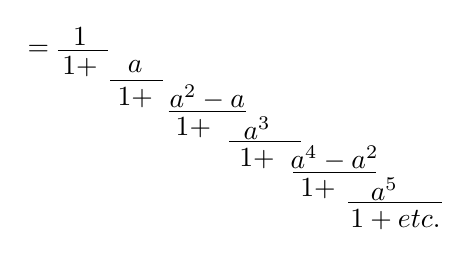
\begin{tikzpicture}[x=1em,y=1em]
\node[inner sep=0] at (-1.5,-.5) {\(=\)};
\node[inner sep=0] at (0,0) {\(1\)};
\draw (-.8,-.5)--(1,-.5);
\node[inner sep=0] at (0,-1.1) {\(1+\)};
\node[inner sep=0] at (2,-1.1) {\(a\)};
\draw (1.1,-1.6)--(3,-1.6);
\node[inner sep=0] at (2,-2.2) {\(1+\)};
\node[inner sep=0] at (4.6,-2.2) {\(a^2-a\)};
\draw (3.2,-2.7)--(6,-2.7);
\node[inner sep=0] at (4.1,-3.3) {\(1+\)};
\node[inner sep=0] at (6.4,-3.3) {\(a^3\)};
\draw (5.4,-3.8)--(8,-3.8);
\node[inner sep=0] at (6.4,-4.4) {\(1+\)};
\node[inner sep=0] at (9.2,-4.4) {\(a^4-a^2\)};
\draw (7.7,-4.9)--(10.7,-4.9);
\node[inner sep=0] at (8.6,-5.5) {\(1+\)};
\node[inner sep=0] at (11,-5.5) {\(a^5\)};
\draw (9.7,-6)--(13.1,-6);
\node[inner sep=0] at (11.4,-6.6) {\(1+\text{etc.}\)};
\end{tikzpicture}
\end{center}
\indent Unde facile omnes series, ubi exp[onentes] ser[iem] sec[undi] ordinis constituunt, transformantur.
\par\noindent\hfill[1797] Febr. 16.

\medskip\begingroup\small
\indent Die »Propositio penultima« der ersten Seite des \textit{Tagebuchs}, auf die hier Bezug genommen wird, ist das erste Beispiel der Notiz Nr. 7 vom 24. Mai 1796, das für \(a=2\) aus der hier angegebenen Formel hervorgeht. Eine Umformung, die der hier von \textsc{Gauss} aufgezeichneten nahe verwandt ist, findet sich ohne Beweis in einem \textit{Theorema} betitelten Aufsatze von G. \textsc{Eisenstein}\footnote{\textsc{Crelles} Journal f. Mathematik \textbf{29}, 1846, S. 96, Mathematische Abhandlungen von G. \textsc{Eisenstein}, Berlin 1847, S. 175; vergl. auch die zweite Fußnote auf der folgenden Seite.}; beide Umformungen sind als besondere Fälle in einer Gleichung enthalten, die \textsc{Eisenstein} in der Abhandlung \textit{Théorèmes sur les formes cubiques etc.}\begingroup\renewcommand{\thefootnote}{**)}\footnote{\textsc{Crelles} Journal f. Mathematik \textbf{27}, 1844, S. 75, siehe besonders S. 78.}\endgroup ebenfalls ohne Beweis angegeben hat. Ein Beweis dieser \textsc{Eisenstein}schen Gleichung kann aus einem Briefe von \textsc{Stieltjes} an \textsc{Hermite}\begingroup\renewcommand{\thefootnote}{***)}\footnote{Siehe \textit{Correspondance d’Hermite et de Stieltjes} II, Paris 1905, S. 423—425, vergl. auch das Briefbruchstück Nr. 387, S. 340.}\endgroup entnommen werden. Die \textsc{Gauss}sche Umformung ergibt sich in folgender Weise aus den oben S. 492 in der Bemerkung zu der Notiz Nr. 7. angegebenen allgemeinen Formeln. Setzt man daselbst in (3) und (6)
\[
c_0=r^{\frac14},\quad c_1=r^{(\frac12+1)^2},\quad c_2=r^{(\frac12+2)^2},\quad c_3=r^{(\frac12+3)^2},\quad\ldotp\,\ldotp\,\ldotp,
\]
\noindent so ist
\[
\begin{aligned}
A_n&=r^{\frac12n(\frac12+2n-2)}\bigl|r^{(i+k-2)^2}\bigr|&\qquad(i,k&=1,2,\ldotp\,\ldotp\,\ldotp,n),\\
B_n&=r^{\frac32n(\frac32+2n-2)}\bigl|r^{(i+k-2)^2}\bigr|&\qquad(i,k&=1,2,\ldotp\,\ldotp\,\ldotp,n),
\end{aligned}
\]
\noindent und für die als Faktor auftretende Determinante findet man\begingroup\renewcommand{\thefootnote}{\(\dagger\))}\footnote{Vergl. \textsc{Stieltjes}, a. a. O. S. 424, Gleichung (\(\gamma\)).}\endgroup
\[
\bigl|r^{(i+k-2)^2}\bigr|=r^{n(n-1)^2}(r^2-1)^{n-1}(r^4-1)^{n-2}\ldotp\,\ldotp\,\ldotp(r^{2n-2}-1).
\]
\noindent Die Ausdrücke (5) und (4) oben S. 492 ergeben also
\[
b_0=r^{\frac14},\quad b_{2n}=r^{2n}(r^{2n}-1),\quad b_{2n+1}=r^{4n+2}\qquad(n=0,1,2,\ldotp\,\ldotp\,\ldotp),
\]
\noindent was nach Unterdrückung des Faktors \(r^{\frac14}\) in Reihe und Kettenbruch für \(x=1,\ r^2=a\) mit der Forme
\par\vfill\noindent X 1.\hfill65
\par\endgroup

\clearpage\SourceLeaf{543}\ArithmeticHead{514}{L}{TAGEBUCH MIT ERLÄUTERUNGEN.}
\begingroup\small
\noindent von \textsc{Gauss} übereinstimmt. Reihe und Kettenbruch von \textsc{Gauss} konvergieren\footnote{Vergl. \textsc{Eisenstein}, Mathem. Abhandlungen, S. 176.} für \(|a|<1\), sie sind also in dem ersten Beispiele der Nr. 7, wo \(a=2\) ist, beide divergent.

\indent Die Tagebuchaufzeichnung, von der hier die Rede ist, stellt das älteste \textls[120]{unmittelbare} Zeugnis dafür dar, daß \textsc{Gauss} sich mit den Potenzreihen beschäftigt hat, deren Exponenten eine arithmetische Reihe zweiter Ordnung bilden, vergl. die Bemerkungen oben S. 262, 266 und den in der zweiten Abteilung dieses Bandes abgedruckten Aufsatz »Über \textsc{Gauss}' Arbeiten zur Funktionentheorie«.

\indent \textsc{Eisenstein} ist im Juli 1844 nach Göttingen gekommen (siehe \textit{Briefwechsel zwischen Gauss und Schumacher} IV, Altona 1862, S. 265, 266); der vom Dezember 1843 datierte Aufsatz im 27. Bande des \textsc{Crelle}schen Journals ist also sicher nicht unmittelbar von \textsc{Gauss} beeinflußt. Dagegen könnte dem \textit{Theorema} im 29. Bande des Journals eine persönliche Anregung von \textsc{Gauss} vorangegangen sein; man ist versucht, die einleitenden Worte\begingroup\renewcommand{\thefootnote}{**)}\footnote{»Invenit vir clarissimus \textsc{Gauss} [\textit{Summatio quarundam serierum singularium}, 1811, art. 8., Werke II, S. 20] aequalitatem inter duas expressiones abstrusiores hancce
\[
1+x+x^3+x^6+x^{10}+\text{etc.}=\frac{1-x^2}{1-x}.\frac{1-x^4}{1-x^3}.\frac{1-x^6}{1-x^5}.\frac{1-x^8}{1-x^7}\ \text{etc.}
\]
\noindent Non minus memorabilis videatur eiusdem seriei evolutio sequens
\begin{center}
\begin{tikzpicture}[x=1em,y=1em]
\node[anchor=east,inner sep=0] at (-1.2,-.5) {\(1+x+x^3+x^6+x^{10}+\text{etc.}=\)};
\node[inner sep=0] at (0,0) {\(1\)};
\draw (-.9,-.5)--(1,-.5);
\node[inner sep=0] at (0,-1.1) {\(1-\)};
\node[inner sep=0] at (2,-1.1) {\(x\)};
\draw (1.1,-1.6)--(3,-1.6);
\node[inner sep=0] at (2,-2.2) {\(1-\)};
\node[inner sep=0] at (4.5,-2.2) {\(x^2-x\)};
\draw (3.2,-2.7)--(5.8,-2.7);
\node[inner sep=0] at (4.5,-3.3) {\(1-\text{etc.}\)};
\node[anchor=west,inner sep=0] at (6,-2.7) {«};
\end{tikzpicture}
\end{center}
}\endgroup geradezu für die Wiedergabe einer von \textsc{Gauss} getanen Äußerung zu halten.
\par\noindent\hfill\textsc{Klein.\quad Schlesinger.}
\par\endgroup
